% This must be in the first 5 lines to tell arXiv to use pdfLaTeX, which is strongly recommended.
\pdfoutput=1
% In particular, the hyperref package requires pdfLaTeX in order to break URLs across lines.

\documentclass[11pt]{article}

% Remove the "review" option to generate the final version.
\usepackage[]{acl}

% Standard package includes
\usepackage{times}
\usepackage{latexsym}

% For proper rendering and hyphenation of words containing Latin characters (including in bib files)
\usepackage[T1]{fontenc}
% For Vietnamese characters
% \usepackage[T5]{fontenc}
% See https://www.latex-project.org/help/documentation/encguide.pdf for other character sets

% This assumes your files are encoded as UTF8
\usepackage[utf8]{inputenc}
\usepackage{subcaption}
\usepackage{graphicx}
\usepackage{balance}

% This is not strictly necessary, and may be commented out,
% but it will improve the layout of the manuscript,
% and will typically save some space.
\usepackage{microtype}

\newcommand{\multiref}[2]{\ref{#1}-\ref{#2}}

% If the title and author information does not fit in the area allocated, uncomment the following
%
%\setlength\titlebox{<dim>}
%
% and set <dim> to something 5cm or larger.

\title{Vocabulary Transfer for Biomedical Texts: \\
Add Tokens if You Can Not Add Data}

% Author information can be set in various styles:
% For several authors from the same institution:
% \author{Author 1 \and ... \and Author n \\
%         Address line \\ ... \\ Address line}
% if the names do not fit well on one line use
%         Author 1 \\ {\bf Author 2} \\ ... \\ {\bf Author n} \\
% For authors from different institutions:
% \author{Author 1 \\ Address line \\  ... \\ Address line
%         \And  ... \And
%         Author n \\ Address line \\ ... \\ Address line}
% To start a seperate ``row'' of authors use \AND, as in
% \author{Author 1 \\ Address line \\  ... \\ Address line
%         \AND
%         Author 2 \\ Address line \\ ... \\ Address line \And
%         Author 3 \\ Address line \\ ... \\ Address line}



\author{Priyanka Singh \\
Higher School of Economics\\
St. Petersburg, Russia\\
\And
Vladislav Mosin\\
LEYA lab,\\
Higher School of Economics\\
St. Petersburg, Russia\\
\And
Ivan P. Yamshchikov\\
CAIRO, THWS\\
W\"{u}rzburg, Germany\\
\texttt{ivan.yamshchikov@thws.de}
}



\begin{document}
\maketitle
\begin{abstract}

Working within specific NLP subdomains presents significant challenges, primarily due to a persistent deficit of data. Stringent privacy concerns and limited data accessibility often drive this shortage. Additionally, the medical domain demands high accuracy, where even marginal improvements in model performance can have profound impacts. In this study, we investigate the potential of vocabulary transfer to enhance model performance in biomedical NLP tasks. Specifically, we focus on vocabulary extension, a technique that involves expanding the target vocabulary to incorporate domain-specific biomedical terms. Our findings demonstrate that vocabulary extension, leads to measurable improvements in both downstream model performance and inference time.

%Working with specific NLP subdomains, particularly in the medical field is challenging. One of the primary challenges is a constant deficit of data, which arises from several factors including privacy concerns or limited accessibility. Additionally, medical domain has critical accuracy requirements where a small improvement in model performance has significant impacts. In this work, we explore how vocabulary transfer can enhance model performance on medical NLP tasks. We demonstrate the vocabulary transfer and in particular vocabulary extension, by expanding the target vocabulary to include medical domain specific terms, can bring tangible improvements both in terms of the downstream model performance and inference time.


 %In the paper, a positive correlation is observed between the number of domain-specific tokens and classifier accuracy. This shows that model performance is improved by increasing the vocab size. This usually improves the resulting performance of the model, and in the paper, we demonstrate that with the increase in number of tokens by vocabulary transfer is especially beneficial for medical text processing. Using  different medical natural language processing datasets, we show vocabulary transfer to provide increase in classifier accuracy as the size to tokens increases.
\end{abstract}
%%%%%%%%%%%%%%%%%%%%%%%%%%%%%%%%%%%%%%%%%%%%%%%%%%%%%%%%%%%%%%%%%%%%%%%%%%%%%%%%%%%%%%%%%
\section{Introduction}

 The Transformer architecture, introduced by \citet{vaswani2017attention}, has revolutionized natural language processing across various domains. In the biomedical field, several Transformer-based models have been specifically tailored for biomedical corpora, including BioBERT \cite{lee2020biobert}, PubMedBERT \cite{gu2021domain}, ClinicalBERT \cite{Huang2019ClinicalBERT}, and MedGPT \cite{Zuo2019MedGPT}, among others. The complexity of tokenization in biomedical texts arises from multiple factors. Biomedical language often diverges significantly from general English in both syntax and lexicon, frequently incorporating complex compound terms, non-standard abbreviations, and specialized terminologies that reflect the field's dynamic and rapidly evolving nature. Biomedical literature often includes acronyms, abbreviations, digits, internal capitalization, special characters, and structured information like medical codes and timestamps.

%Transfer learning is a machine learning technique that leverages knowledge gained from one task to enhance performance on a related task. The widespread adoption of transfer learning has generated significant interest in refining and optimizing these techniques. Consequently, numerous strategies and methods have been developed to make the transfer process more efficient and effective, as explored by \citet{raffel2020exploring}.

%The transformer introduced in  \citet{vaswani2017attention}. Some transformer models are  introduced specially for biomedical corpora as BioBERT \cite{JinhyukLee2019}, PubMedBERT ,  ClinicalBERT \cite{Huang2019ClinicalBERT} , MedGPT \cite{Zuo2019MedGPT} and more. The complexity of biomedical tokenization arises from several factors. Firstly, the language used in biomedical texts frequently diverges from general English in terms of syntax and lexicon, often including complex compound terms, non-standard abbreviations, and diverse terminologies that reflect the rapidly evolving nature of the field. Biological publications often include acronyms, abbreviations, digits, capitalized letters inside words, Latin and Greek characters, Roman numerals, units of measurement, lists, enumerations, tabular data, hyphens, and other special symbols commonly used in
%biological language. Furthermore, medical texts often contain structured information, such as patient demo- graphics, medical codes (e.g., ICD-10, CPT), and timestamps.  Transfer learning is a technique in machine learning in which knowledge learned from a task is re-used in order to boost performance on a related task. This widespread use has sparked a lot of interest in improving transfer learning techniques. As a result, many different strategies and methods to make the transfer process more efficient and effective were developed \citet{raffel2020exploring}. 

This paper explores applicability of vocabulary transfer introduced in \citet{mosin2023fine} to biomedical domain. Traditionally, language models employ the same tokenization method during both initial training and subsequent fine-tuning, typically encompassing thousands of tokens. These tokens can vary from subword units to full words. However, \citet{mosin2023fine} propose that developing a new, task-specific tokenization strategy during the fine-tuning stage may significantly improve model performance.

Vocabulary transfer becomes particularly particularly advantageous when the fine-tuning dataset differs substantially from the one used in initial training. Research in biomedical tokenization has highlighted several problematic cases that exemplify the challenges inherent in this domain, for detailed examples see \citet{Lopez2015}. 

%These challenges include hyphenated terms, abbreviations, chemical symbols, and genetic information, each of which may be tokenized inconsistently. For instance, tokenizing phrases such as "3-year-old patient" or "anti-inflammatory drugs" requires decisions about whether hyphens should be treated as delimiters or as integral parts of tokens. Similarly, medical terms like "Costochondritis," which refers to chest pain caused by inflammation of the cartilage connecting the ribs to the breastbone, present challenges due to their rarity in general English. Another example is "pneumonoultramicroscopicsilicovolcanoconiosis," an exceptionally long medical term that presents significant challenges for tokenization models trained on general text corpora.

%Accurate tokenization in the biomedical domain is crucial for correctly interpreting complex medical language, and it significantly impacts the performance of downstream applications such as clinical decision support systems, disease surveillance, and biomedical research. In these contexts, better transfer of existing knowledge through optimized tokenization strategies could be particularly beneficial, enabling more effective processing of medical texts and the extraction of meaningful information. 


Though in this paper we experiment with biomedical data we believe that similar vocabulary extension approach would be beneficial for other NLP domains where the data is scarce. \cite{gee2022fast} has demonstrated the vocabulary transfer could be beneficial for model compression in business applications. \cite{yamshchikov2022bert} has shown the benefits of vocabulary transfer when using the model trained on the modern Greek texts on the historical texts in ancient Greek, while \cite{remy2024trans,alexandrov2024mitigating} show its benefits when working with low-resource languages. This paper demonstrates that vocabulary transfer is applicable to biomedical texts and can bring certain benefits. We also demonstrate that increasing vocabulary size, i.e. {\em vocabulary extension}, during vocabulary transfer significantly improves downstream performance. We believe this result is not limited to biomedical data but would hold on any other specific domain.
%By tailoring the tokenization process to the specific task or dataset, with an expanded token set, the model may better adapt to the unique characteristics of the new data, thereby enhancing its processing capabilities.

%This paper demonstrates that with the increase in vocabulary size, vocabulary transfer \cite{mosin2023fine} helps in natural language processing in the biomedical domain.  Traditionally, language models use the same tokenization method for both initial training and later fine-tuning, typically involving thousands of tokens. These tokens can range from small parts of words to longer tokens that represent entire words. However, \citet{mosin2023fine} propose that creating a new, task-specific tokenization for the fine-tuning stage could improve the model's performance. This approach could be particularly valuable when the dataset used for fine-tuning is very different from the one used for initial training. By customizing the tokenization to the specific task or dataset with the larger number of tokens, the model might better adapt to the unique characteristics of the new data it's processing.


%Vocabulary transfer seems especially relevant when the dataset used for fine-tuning has many words and parts of words, which are rare in the pretraining dataset and frequent in the downstream one. Research in biomedical tokenization has identified numerous problematic cases that typify the challenges inherent in the domain. These include issues with hyphenated terms, abbreviations, chemical symbols, and genetic information, each of which may be tokenized inconsistently depending on the tokenizer’s configuration and the specific rules it follows as said by \cite{Díaz-Lopez2015}. For example, tokenizing a phrase like "3-year-old patient" or "anti-inflammatory drugs" involves decisions about whether to treat hyphens as delimiters or parts of tokens or "Costochondritis" which means chest pain caused by the inflammationone more example is in medical terms like of the cartilage that connects the ribs to the breastbone, which can significantly affect the interpretation of the text as it is not a very common word in English. One more example of medical terms "pneumonoultramicroscopicsilicovolcanoconiosis" can be exceptionally long and pose difficulties for traditional tokenization methods. By systematically processing medical texts and extracting meaningful information, tokenization enables a wide range of applications, including clinical decision support systems, disease surveillance, and biomedical research. In this case, better transfer of the existing knowledge could be especially relevant. 


%We experiment with text classification as a downstream task in biological domain \cite{mujtaba2019clinical, gao2021limitations, hughes2017medical} on two datasets: OHSUMED \cite{hersh1994ohsumed} - medical dataset for classification cardiovascular diseases and Kaggle Medical Texts Dataset\footnote{https://www.kaggle.com/chaitanyakck/medical-text} - medical dataset for classification different conditions of a patient: digestive system diseases, cardiovascular diseases, neoplasms, nervous system diseases, and general pathological conditions. We demonstrate that larger number of tokens improves the classifier accuracy with MLM for downstream medical classification task.

%%%%%%%%%%%%%%%%%%%%%%%%%%%%%%%%%%%%%%%%%%%%%%%%%%%%%%%%%%%%%%%%%%%%%%%%%%%%%%%%%%%%%%%%%%%
\section{Vocabulary transfer}

In their study, \citet{mosin2023fine} introduce the concept of {\em vocabulary transfer}. Let $V$ denote the original vocabulary obtained during the pretraining phase, comprising $M$ tokens denoted as $\{t_k, v_k\}$, where $t_k$ is a text segment forming a token, and $v_k$ is the corresponding embedding for that token. Then $\widetilde{V}$ represents the new vocabulary utilized during fine-tuning, consisting of $N$ tokens denoted as $\{\widetilde{t}_k, \widetilde{v}_k\}$, where $\widetilde{t}_k$ is a text segment forming a new token, and $\widetilde{v}_k$ is its corresponding embedding. This customized tokenization strategy in the fine-tuning phase facilitates improved model performance on specific tasks or datasets.

%In their study, \citet{mosin2023fine} introduce the concept of {\em vocabulary transfer}. To clarify this concept, they use specific notation: $V$ represents the original vocabulary obtained during the pretraining phase, consisting of $M$ tokens denoted as $\{t_k, v_k\}$, where $t_k$ is a piece of text forming a token and $v_k$ is the corresponding embedding for that token. In contrast, $\widetilde{V}$ represents the new vocabulary used during fine-tuning, containing $N$ tokens expressed as $\{\widetilde{t}_k, \widetilde{v}_k\}$, where $\widetilde{t}_k$ is a piece of text that forms a new token and $\widetilde{v}_k$ is its corresponding embedding. This customized tokenization strategy during the fine-tuning phase allows for improved model performance on specific tasks or datasets.

%In this paper, we aim to optimize the vocabulary transfer model and evaluate its impact on classifier accuracy using vocabulary transfer in conjunction with masked language modeling (MLM). We employ two token initialization methods: matched and averaged transfers. The matched approach assigns the embedding of an existing token from the original vocabulary to a new token if there is an exact match. In contrast, the averaged method divides new tokens into segments corresponding to tokens in the original vocabulary and initializes them using the average of the embeddings of the constituent tokens. Both strategies are designed to preserve the semantic meaning of the original tokens while adapting to the new, domain-specific vocabulary.

%In this paper, we try to optimize the vocabulary transfer model and test the change in classifier accuracy using vocabulary transfer with MLM. Two token initialization method used are matched and averaged transfers. The matched approach assigns the embedding of an existing token in the old vocabulary to a new token if they coincide exactly. The averaged method splits new tokens into partitions of old tokens and initializes them using the average of the embeddings of the constituent tokens. Both strategies aim to preserve the semantic meaning of the original tokens while adapting to new, domain-specific vocabulary.

%In the biomedical domain, increasing vocabulary size frequently results in improved classifier accuracy, particularly for tasks such as biomedical entity recognition and clinical text classification. This improvement is primarily due to the model's enhanced capacity to capture and represent nuanced and highly specific biomedical terminology, which is essential for the accurate interpretation of clinical texts.

%In the medical domain, increasing the vocabulary size often leads to improved classifier accuracy, especially for tasks like medical entity recognition and clinical text classification. This improvement is largely attributed to the model's enhanced ability to capture and represent the nuanced and highly specific medical terms that are crucial for accurate interpretation of clinical texts.



%The relationship between vocabulary size and model performance in natural language processing is complex and multifaceted. On one hand, increasing the vocabulary size generally leads to improved classifier accuracy, particularly for masked language modeling (MLM) tasks. This is because larger vocabularies allow for more nuanced and precise representations of linguistic concepts, potentially leading to higher accuracy in predicting masked tokens. However, this increase in vocabulary size comes with a trade-off in terms of inference time. Larger vocabularies typically result in faster inference times, as fewer tokens need to be processed during prediction. This paradoxical situation arises because while a larger vocabulary improves the model's ability to capture subtle distinctions in language, it also reduces the computational complexity required for each prediction. Furthermore, certain techniques like vocabulary transfer and fine-tuning can further optimize this balance, allowing for even more effective use of increased vocabulary sizes. Ultimately, the optimal vocabulary size depends on the specific task and available computational resources, highlighting the importance of carefully managing these competing factors in NLP model design.

To transfer pretrained knowledge from existing tokens to new, corpus-specific tokens, a heuristic token-matching procedure can be employed. In this paper, we evaluate two token initialization heuristics. First, if a token in the new vocabulary directly matches a token in the original vocabulary, its corresponding embedding is assigned to the new token. We refer to this approach as \textit{matched} vocabulary transfer. Additionally, some new tokens may be decomposable into partitions of multiple tokens from the original vocabulary. For each such token in the new vocabulary, we generate all possible partitions comprising tokens from the original vocabulary and select the partition with the minimal number of tokens. If multiple partitions have the same number of tokens, we choose the one containing the longest token. The embedding for the new token is then initialized by averaging the embeddings of the tokens in the selected partition. We refer to this approach as \textit{averaged} transfer. These methods correspond to those described by \citet{mosin2023fine}, where \textit{matched} aligns with the "Match Old Tokens" strategy and \textit{averaged} corresponds to "VIPI".

%To transfer pretrained knowledge about old tokens to the new, corpus-specific tokens, one could have some heuristic procedure of token matching. In this paper, we test two token initialization heuristics. First, if a token in the new vocabulary coincides with some token in the old one, we can assign its old embedding. We denote this vocabulary transfer as {\em matched}. At the same time, some of the new tokens could be split into a partition of several tokens from the original tokenization. For every such token in a new vocabulary, we build all possible partitions that consist of the old vocabulary tokens. We choose a partition with a minimal number of tokens out of these partitions. If there is more than one partition with the same amount of tokens, we choose the one that includes the most extended token. We initialize the corresponding token from the new vocabulary with the old vocabulary embeddings averaged over the chosen partition for every selected partition. We call this transfer {\em averaged}. These methods completely match with ones described in \cite{mosin2023fine}, {\em matched} is Match Old Tokens and {\em average} is VIPI \cite{mosin2023fine}

%%%%%%%%%%%%%%%%%%%%%%%%%%%%%%%%%%%%%%%%%%%%%%%%%%%%%%%%%%%%%%%%%%%%%%%%%%%%%%%%%%%%%%%
\section{Data}

We conduct experiments on text classification as a downstream task within the biological domain \cite{mujtaba2019clinical, gao2021limitations, hughes2017medical} using two datasets: OHSUMED \cite{hersh1994ohsumed}, a medical dataset for the classification of cardiovascular diseases, and the Kaggle Medical Texts Dataset\footnote{https://www.kaggle.com/chaitanyakck/medical-text}, which classifies various patient conditions including digestive system diseases, cardiovascular diseases, neoplasms, nervous system diseases, and general pathological conditions. The downstream dataset was split into 80$\%$, 10$\%$ dev, and 10$\%$ test. Our results demonstrate that increasing the number of tokens enhances classifier accuracy when using masked language modeling (MLM) and vocabulary transfer before downstream classification tasks.

Table \ref{tab:data} summarizes the parameters of the datasets that we experiment with.


\begin{table}[h]
\centering
\begin{tabular}{lrr}
 Dataset & Numer of  & Number of  \\
 & Records & Labels\\
\hline
OHSUMED & 13 929 & 23 \\
Kaggle & 28 880 & 5 \\
\hline
\end{tabular}
\caption{Parameters of the datasets used for experiments with the number of records and the number of labels.}
\label{tab:data}
\end{table}


\begin{figure}[h]
		\centering
    	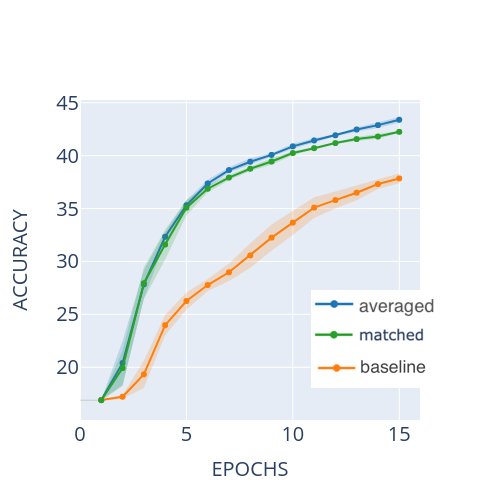
\includegraphics[scale=0.4]{ohsumed_32k_1e-6.png}
    	\caption{Performance on Ohsumed data, vocabulary size is 32 000}
    	\label{fig:len_lr}
\end{figure}

\begin{figure}[h]
		\centering
    	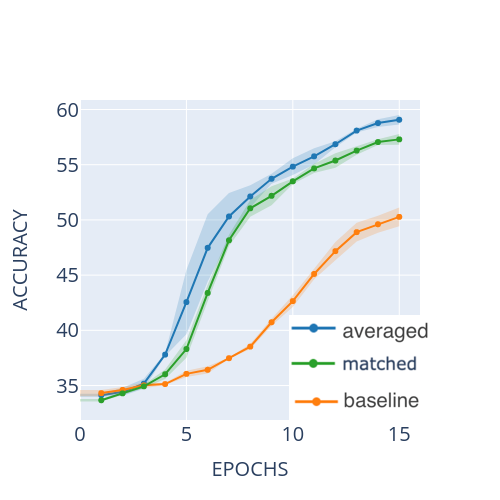
\includegraphics[scale=0.4]{illness_32k_1e-6.png}    
    	\caption{Performance on Kaggle Medical dataset, vocabulary size is 32 000}
    	\label{fig:kmd}
\end{figure}





Table \ref{tab:label table} summarizes the total number of frequencies in each label in Kaggle dataset.
\begin{table}[htbp]
\centering 

\begin{tabular}{c| c c c c c}
    \hline
    \textbf{Label} & 1 & 2 & 3 & 4 & 5 \\
    \hline
    \textbf{Frequency} & 3163 & 1494 & 1925 & 3051 & 4805\\
    \hline
\end{tabular}
\caption{Number of Text Data in each Label of Kaggle dataset }
\label{tab:label table}
\end{table}

%%%%%%%%%%%%%%%%%%%%%%%%%%%%%%%%%%%%%%%%%%%%%%%%%%%%%%%%%%%%%%%%%%%%%%%%%%%%%%%%%%%%%%%%%%
\section{Experiments}

We conducted a series of experiments using the base version of the BERT model on various medical datasets. Initially, we explored the adoption of a new, dataset-specific vocabulary through an intermediary masked language modeling (MLM) step, involving pretraining on the downstream dataset with updated tokenization. Subsequently, we performed multiple experiments with different parameters and compared the results to a baseline approach, which involved simple fine-tuning on the downstream dataset without applying vocabulary transfer or altering the initial tokenization. This baseline serves as a reference point in our experimental analysis.

%We run a series of experiments with the base version of the BERT model on different medical datasets. First, we discuss adopting new dataset-specific vocabulary via an intermediary MLM step, pretraining on a downstream dataset with new tokenization. Then we run several experiments with various parameters and compare results with simple finetuning on the downstream dataset without vocabulary transfer and initial tokenization, we call this {\em Baseline} in our experiments.

\subsection{Fine-tuning Transferred Vocabulary and Change in Classifier Accuracy}

In these experiments, we investigated the limitations of simple token matching in vocabulary transfer and assessed the impact of masked language modeling (MLM) step on the overall performance after vocabulary transfer. We also experiment with the size of the final vocabulary.

First, merely assigning new embeddings to tokens is insufficient for enhancing model performance. Table \ref{tab:classifier_accuracy} presents the relative change in accuracy of downstream classifiers for a medical dataset with five classes without intermediate MLM step and with it. It stands to reason that MLM is important since it allows the model to adapt to new data-set specific tokenization.

%Figures \ref{fig:len_lr}, \ref{fig:kmd} show significant improvements in vocabulary transfer methods compared to the baseline.

%In our experiment, we explored the limitations of simple token matching in vocabulary transfer and tested a more advanced method using masked language modeling (MLM). We realized that merely assigning new embeddings to tokens wasn't sufficient to improve our model's performance. To address this, we implemented a two-stage process. First, we applied an MLM to our target dataset, which was crucial for helping our model adapt to the specific language and patterns of the new domain. After this intermediate step, we trained our final classifier. To evaluate the effectiveness of our approach, we compared two methods: averaged vocabulary transfer without the MLM step and averaged vocabulary transfer with the MLM step. Our results indicated that incorporating the MLM step made a significant difference, enabling our model to better understand the nuances of the new domain compared to just matching tokens. This experiment highlighted that vocabulary transfer is more complex than we initially thought; simply matching tokens isn't enough to achieve optimal results in NLP tasks. The MLM step proved to be a better step, allowing our model to grasp the unique characteristics of the target domain effectively.

Table \ref{tab:classifier_accuracy} also llustrates the impact of vocabulary extension. Indeed, reducing the vocabulary size from 16,000 to 8,000 tokens results in a minor accuracy decrease of 0.26\% for VIPI alone, while the MLM+VIPI approach experiences a more pronounced decline of 4.03\%. In contrast, increasing the vocabulary size to 32,000 tokens leads to a 1.24\% decrease in accuracy for VIPI alone, but a 2.16\% improvement with the MLM+VIPI method. This trend continues at 64,000 tokens, where VIPI alone decreases by 3.45\%, whereas the MLM+VIPI approach results in a 2.51\% improvement.

These findings suggest that expanding vocabulary size enhances model performance. This indicates that MLM effectively prepares the model to leverage larger vocabularies in domain-specific tasks.


%The table \ref{tab:classifier_accuracy} shows the relative change in accuracy of downstream classifiers for medical dataset with 5 classes that changes in vocabulary size affect classifier accuracy under two training scenarios: using Vocabulary Initialization with Partial Inheritance (VIPI) alone and a combined approach of Masked Language Model (MLM) fine-tuning followed by VIPI. Reducing the vocabulary size from 16,000 to 8,000 tokens results in a minor accuracy decrease of 0.26\% for VIPI alone, while the MLM+VIPI approach sees a more significant drop of 4.03\%. Conversely, increasing vocabulary size to 32,000 tokens leads to a 1.24\% decrease for VIPI alone, but a 2.16\% improvement for the MLM+VIPI method. This trend continues with 64,000 tokens, where VIPI alone decreases by 3.45\%, while MLM+VIPI improves by 2.51\%. These results indicate that expanding vocabulary size, particularly when paired with MLM pre-fine-tuning, enhances model performance, suggesting that MLM effectively prepares the model to utilize larger vocabularies in domain-specific tasks.

\begin{table*}[t]
\centering
\begin{tabular}{l|c|c}
\hline
Vocabulary size & Change of accuracy & Change of accuracy\\
 & transfer only & transfer and MLM \\
\hline
16000 $\rightarrow$ 8000 & \textbf{-0.26\%} & -4.03\% \\
16000 $\rightarrow$ 32000 & -1.24\% & +2.16\% \\
16000 $\rightarrow$ 64000 & -3.45\% & \textbf{+2.51\%} \\
\hline
\end{tabular}

\caption{Relative change in downstream classifier accuracy and the impact of corpus-specific tokenization on a Kaggle medical dataset compared to standard fine-tuning with 16,000 tokens.}
\label{tab:classifier_accuracy}
\end{table*}


\subsection{Vocabulary Size and Inference time} \label{sec:sm}

In the medical domain, inference time might be critically important as it directly influences the speed and efficiency of healthcare analysis. Since patient data is highly sensitive and medical emergencies might occur in various conditions, local inference on diagnostic device rather than server-based inference might be vastly beneficial. This makes inference speed and efficiency paramount. Rapid inference facilitates real-time decision-making, swift processing of medical data, and timely responses in emergencies. Moreover, efficient inference optimizes resource utilization, accelerates patient care workflows, and enhances the overall experience for healthcare professionals. Faster inference times contribute to a more responsive, accessible, and effective healthcare system, ultimately improving patient care and outcomes, particularly in time-sensitive medical analyses.

Vocabulary size has a direct impact on inference time. In our experiment, as shown in Figure \ref{fig:inf_time}, we found that using a classifier with a larger vocabulary leads to increased inference time if the intermediary MLM step was not performed. However, as illustrated in Figure \ref{fig:mlm_inf_time}, incorporating a masked language model (MLM) training after vocabulary transfer results in decreased inference time as the vocabulary size increases.While larger vocabulary sizes generally increases inference time incorporating an MLM step allows the efficient handling of domain-specific vocabularies.This optimization reduces the computational burden during tokenization. Naturally, MLM enhances compression enabling the moder to process domain-specific data more efficiently throughout the all stages such as tokenization, embedding and final prediction generation.



%In the medical field, inference time is very important because it has a direct effect on how quickly and effectively healthcare analysis is delivered. Fast inference makes it possible to help people make decisions in real time, handle medical data quickly, and act quickly in emergencies. Efficient inference also makes better use of resources, speeds up the process of seeing patients, and improves the experience for healthcare workers. Faster inference time makes healthcare more responsive, easy to access, and effective, which improves patient care and results in medical analysis where time is of the essence. The vocabulary size—the range of words the model can recognize and process—directly influences inference time.In our experiment,in fig \ref{fig:inf_time} we found that by using only classifier with the larger vocabulary, the inference time for the model also increases. However,by using masked language model with vocabulary transfer, in fig \ref{fig:mlm_inf_time} we also observed that with a larger vocabulary, the inference time actually decreases, improving the model's ability to transfer vocabulary knowledge. This enhancement enables the model to handle more medical data efficiently during key steps like embedding, tokenization, and final prediction generation.

\begin{figure}[h]
		\centering
    	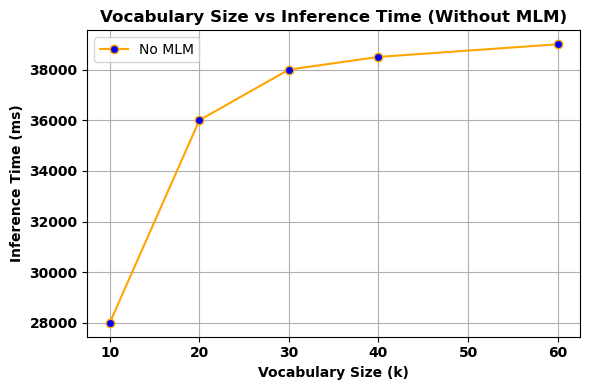
\includegraphics[scale=0.5]{clf_plot.png}    
    	\caption{Change of classifier accuracy on Kaggle Medical dataset, inference time with respect to vocabulary size + VIPI only. }
    	\label{fig:inf_time}
\end{figure}

\begin{figure}[h]
		\centering
    	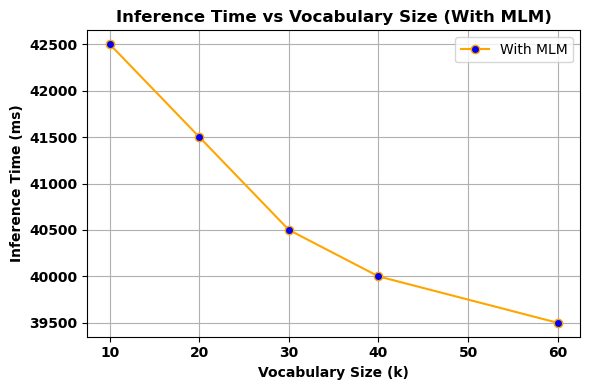
\includegraphics[scale=0.5]{mlm_plot.png}    
    	\caption{Relative change in accuracy of downstream classifiers on Kaggle Medical dataset, inference time with respect to vocabulary size after MLM and VIPI}
    	\label{fig:mlm_inf_time}
\end{figure}


%%%%%%%%%%%%%%%%%%%%%%%%%%%%%%%%%%%%%%%%%%%%%%%%%%%%%%%%%%%%%%%%%%%%%%%%%%%%%%%%%%%%%%%%%%%%%%
\section{Discussion}

Several key aspects of vocabulary transfer for medical texts are evident from our analysis. First, the intermediary MLM step proves beneficial. Our further experiments show that even when applied to pre-existing tokenization, MLM on downstream data before training the classifier provides certain benefits. Likely, tokens rare in standard English but essential for medical NLP are better adjusted during this intermediate MLM phase. Additionally, the use of VIPI in conjunction with MLM appears to contribute to increased classifier accuracy especially if the vocabulary is extended.

%Second, as the vocabulary size increases, the inference time for model predictions decreases. 
Our findings also shows that the MLM step not only improves the model's classification performance but also leads to a reduction in inference time. By this we could say that MLM step compresses the token representation and optimizes the model for faster interference, even when the vocabulary size is significantly increased. By optimizing inference time, we can develop more efficient and responsive models. While more advanced and robust procedures may exist, our findings suggest that even a straightforward approach to vocabulary transfer in medical NLP can be significantly enhanced by expanding the vocabulary size.

%Finally, averaging tokens that can be represented as a union of those from the original vocabulary, especially with an enlarged vocabulary, tends to yield an additional two percentage points in downstream accuracy.

%One could notice several essential aspects of vocabulary transfer for medical texts. First, the intermediary MLM step is always helpful, even over old predefined tokenization. One could speculate that some tokens that are rare in standard English but are helpful for medical NLP are adjusted through the intermediate MLM step. One could also speculate that by using VIPI with MLM the classifier accuracy increases.

%Second, with the larger tokens the inference time for model prediction reduces.By optimizing inference time we could get more efficient and responsive models. Maybe, there is a better and more robust procedure out there, but it seems that the most straightforward vocabulary transfer for medical NLP can be made better if we provide larger vocabulary.

%Finally, averaging the tokens that could be represented as a union of old ones with the larger vocabulary tends to give two extra percentage points in the downstream accuracy.

%%%%%%%%%%%%%%%%%%%%%%%%%%%%%%%%%%%%%%%%%%%%%%%%%%%%%%%%%%%%%%%%%%%%%%%%%%%%%%%%%%%%%%%%%%%%%

%%%%%%%%%%%%%%%%%%%%%%%%%%%%%%%%%%%%%%%%%%%%%%%%%%%%%%%%%%%%%%%%%%%%%%%%%%%%%%%%%%%%%%%%%%%%%
\section{Conclusion}

%This paper demonstrates that vocabulary transfer could be beneficial for medical natural language processing. We show how different steps of vocabulary transfer affect resulting performance on the task of classification using medical datasets. With the larger vocabulary the model performs better.

This paper demonstrates the potential benefits of vocabulary transfer in medical natural language processing. We analyze the impact of various stages of vocabulary transfer on classification performance using medical datasets. Our findings indicate that increasing the vocabulary size leads to improved model performance.

\section{Limitations}
Our experiments are limited to text classification tasks using the base version of the BERT model tested on several specific datasets. We do anticipate that the proposed approach could be beneficial for other models and subdomains, since vocabulary transfer seem to have demonstrably similar effects in various domains, see \cite{yamshchikov2022bert, alexandrov2024mitigating, gee2022fast}. However, when working with models of bigger scale then BERT the effects of vocabulary transfer might be more or less pronounced.

\section*{Ethics Statement}
This paper complies with the \href{https://www.aclweb.org/portal/content/acl-code-ethics}{ACL Ethics Policy}.

\section*{Acknowledgements}
We would like to thank Mr. Pavel Chizhov and Mr. Alexey Tikhonov for their advice, productive ideas and support.

\bibliography{anthology}
\bibliographystyle{acl_natbib}

\end{document}